\documentclass[12pt]{article}
 
\usepackage[margin=1in]{geometry} 
\usepackage{amsmath,amsthm,amssymb}

\usepackage[brazilian]{babel}
\usepackage[utf8]{inputenc}
\usepackage[T1]{fontenc}
\usepackage{graphicx}         %pacote para incluir figuras tipo eps
\usepackage{xcolor}
\usepackage{float} 
\usepackage{epstopdf}
\usepackage{longtable}
\usepackage{subcaption}

 
 %Matlab code in latex 
\usepackage[final]{listings}
\usepackage{color} %red, green, blue, yellow, cyan, magenta, black, white
\definecolor{mygreen}{RGB}{28,172,0}
\definecolor{mylilas}{RGB}{170,55,241}
\lstdefinestyle{myMatlab}
{
language=matlab,frame=single, basicstyle=\small\ttfamily,breaklines=true,%
morekeywords={matlab2tikz}, keywordstyle=\color{blue}, morekeywords=[2]{1}, keywordstyle=[2]{\color{black}}, commentstyle=\color{mygreen}, stringstyle=\color{mylilas}, identifierstyle=\color{black}, showstringspaces=false,%without this there will be a symbol in the places where there is a space
numbers=left, numberstyle={\scriptsize \color{black}},% size of the numbers
numbersep=9pt, % this defines how far the numbers are from the text
% emph=[1]{for,end,break},emphstyle=[1]\color{red}, %some words to emphasise
% emph=[2]{word1,word2}, emphstyle=[2]{style},
}
 
\newcommand{\N}{\mathbb{N}}
\newcommand{\Z}{\mathbb{Z}}
 
\newenvironment{theorem}[2][Theorem]{\begin{trivlist}
\item[\hskip \labelsep {\bfseries #1}\hskip \labelsep {\bfseries #2.}]}{\end{trivlist}}
\newenvironment{lemma}[2][Lemma]{\begin{trivlist}
\item[\hskip \labelsep {\bfseries #1}\hskip \labelsep {\bfseries #2.}]}{\end{trivlist}}
\newenvironment{exercise}[2][Exercício]{\begin{trivlist}
\item[\hskip \labelsep {\bfseries #1}\hskip \labelsep {\bfseries #2.}]}{\end{trivlist}}
\newenvironment{reflection}[2][Reflection]{\begin{trivlist}
\item[\hskip \labelsep {\bfseries #1}\hskip \labelsep {\bfseries #2.}]}{\end{trivlist}}
\newenvironment{proposition}[2][Proposition]{\begin{trivlist}
\item[\hskip \labelsep {\bfseries #1}\hskip \labelsep {\bfseries #2.}]}{\end{trivlist}}
\newenvironment{corollary}[2][Corollary]{\begin{trivlist}
\item[\hskip \labelsep {\bfseries #1}\hskip \labelsep {\bfseries #2.}]}{\end{trivlist}}
 
\begin{document}
 
% --------------------------------------------------------------
%                         Start here
% --------------------------------------------------------------
 
\title{Exercício 02}
\author{Renan Salles de Freitas\\
CPE 723 - Otimização Natural}
 
\maketitle
 
\begin{exercise}{1.a}
Temos que a distribuição de probabilidade de $X(1)$ é:
\begin{align*}
\textbf{p}_1 &= M\textbf{p}_0
\end{align*}
E ainda:
\begin{align*}
\textbf{p}_2 = M\textbf{p}_1 &= M^2\textbf{p}_0 \\
\textbf{p}_n &= M^n\textbf{p}_0
\end{align*}
Portanto:
\begin{align*}
\textbf{p}_3 &= M^3\textbf{p}_0 \\
\textbf{p}_3 &= \begin{bmatrix}
0.3328 \\ 0.3344 \\ 0.3328
\end{bmatrix}
\end{align*}
\end{exercise}
 
\begin{exercise}{1.b} Supondo que estamos no estado $X(t)$, construímos uma
lista com os possíveis próximos estados, considerando a distribuição de
probabilidade, conforme a matriz de transição de estados $M$:
$X(t+1) = [X(t) \quad 0 \quad 1 \quad 2]$. Sorteamos um índice de zero a quatro
com o MatLab e atualizamos $X(t+1)$. Observe que, dessa forma, a transsição
para o estado o estado atual sempre possui probabilidade $0.5$ e os outros
estados possuem probabilidade $0.25$.
\begin{align}
X(0) &= 1 \\
\nonumber \text{list} &= [0 \quad 1 \quad 2 \quad 1] \\
\nonumber r &= \text{randi}(4) = 3 \\
\nonumber X(1) &= \text{list}(r) = 2  
\end{align}

\begin{align}
X(1) &= 2 \\
\nonumber \text{list} &= [0 \quad 1 \quad 2 \quad 2] \\
\nonumber r &= \text{randi}(4) = 3 \\
\nonumber X(2) &= \text{list}(r) = 2  
\end{align}

\begin{align}
X(2) &= 2 \\
\nonumber \text{list} &= [0 \quad 1 \quad 2 \quad 2] \\
\nonumber r &= \text{randi}(4) = 4 \\
\nonumber X(3) &= \text{list}(r) = 2  
\end{align}

\end{exercise}

\begin{exercise}{1.c} Código MatLab abaixo:
\lstinputlisting[style=myMatlab]{matlab/ex1_c.m} 
% 
% \begin{longtable}{cccc} $\textbf{X(0)}$ & $\textbf{X(1)}$ & $\textbf{X(2)}$ &
% $\textbf{X(3)}$\\ \endfirsthead $\textbf{X(0)}$ & $\textbf{X(1)}$ & $\textbf{X(2)}$ &
% $\textbf{X(3)}$\\
% \endhead
% 2      & 2      & 2      & 1      \\
% 2      & 2      & 0      & 0      \\
% 2      & 0      & 0      & 2      \\
% 2      & 0      & 2      & 0      \\
% 1      & 1      & 1      & 1      \\
% 1      & 1      & 2      & 0      \\
% 2      & 2      & 2      & 2      \\
% 0      & 1      & 0      & 0      \\
% 0      & 0      & 1      & 1      \\
% 1      & 2      & 2      & 2      \\
% 1      & 0      & 0      & 0      \\
% 2      & 1      & 1      & 1      \\
% 2      & 2      & 1      & 2      \\
% 1      & 0      & 2      & 0      \\
% 1      & 0      & 2      & 0      \\
% 2      & 0      & 0      & 2      \\
% 0      & 2      & 0      & 0      \\
% 1      & 0      & 0      & 1      \\
% 1      & 1      & 1      & 1      \\
% 1      & 1      & 1      & 2      \\
% 0      & 0      & 1      & 2      \\
% 2      & 0      & 0      & 2      \\
% 0      & 0      & 0      & 1      \\
% 1      & 1      & 2      & 2      \\
% 0      & 1      & 0      & 2      \\
% 0      & 2      & 2      & 2      \\
% 2      & 1      & 0      & 0      \\
% 1      & 1      & 1      & 2      \\
% 2      & 0      & 1      & 0      \\
% 2      & 2      & 1      & 1      \\
% 2      & 2      & 2      & 0      \\
% 0      & 0      & 0      & 2      \\
% 2      & 2      & 1      & 0      \\
% 0      & 0      & 0      & 1      \\
% 1      & 0      & 2      & 0      \\
% 1      & 2      & 1      & 2      \\
% 1      & 1      & 1      & 0      \\
% 1      & 0      & 2      & 2      \\
% 0      & 1      & 1      & 1      \\
% 1      & 2      & 2      & 1      \\
% 2      & 0      & 2      & 0      \\
% 1      & 0      & 1      & 1      \\
% 2      & 0      & 2      & 2      \\
% 1      & 0      & 1      & 1      \\
% 2      & 0      & 0      & 1      \\
% 2      & 2      & 0      & 2      \\
% 1      & 2      & 0      & 1      \\
% 2      & 1      & 0      & 0      \\
% 1      & 0      & 0      & 1      \\
% 0      & 0      & 0      & 2      \\
% 0      & 1      & 1      & 0      \\
% 2      & 2      & 1      & 2      \\
% 2      & 2      & 2      & 0      \\
% 2      & 2      & 2      & 0      \\
% 2      & 1      & 0      & 0      \\
% 1      & 2      & 1      & 1      \\
% 2      & 0      & 2      & 1      \\
% 1      & 1      & 2      & 1      \\
% 2      & 2      & 2      & 2      \\
% 2      & 1      & 0      & 0      \\
% 2      & 2      & 2      & 2      \\
% 2      & 1      & 0      & 1      \\
% 0      & 2      & 2      & 2      \\
% 2      & 2      & 0      & 1      \\
% 2      & 2      & 0      & 0      \\
% 1      & 1      & 2      & 0      \\
% 0      & 1      & 1      & 1      \\
% 1      & 1      & 1      & 1      \\
% 0      & 0      & 0      & 1      \\
% 0      & 0      & 0      & 0      \\
% 0      & 2      & 2      & 2      \\
% 2      & 1      & 1      & 1      \\
% 2      & 2      & 2      & 2      \\
% 1      & 0      & 2      & 2      \\
% 0      & 0      & 0      & 2      \\
% 2      & 2      & 2      & 2      \\
% 2      & 0      & 1      & 1      \\
% 1      & 1      & 2      & 1      \\
% 1      & 0      & 0      & 0      \\
% 1      & 1      & 1      & 2      \\
% 0      & 1      & 1      & 0      \\
% 0      & 0      & 1      & 1      \\
% 1      & 1      & 2      & 2      \\
% 0      & 0      & 0      & 0      \\
% 1      & 1      & 0      & 0      \\
% 1      & 2      & 1      & 1      \\
% 0      & 0      & 1      & 2      \\
% 0      & 2      & 2      & 1      \\
% 1      & 1      & 1      & 0      \\
% 0      & 2      & 0      & 0      \\
% 1      & 0      & 2      & 2      \\
% 1      & 1      & 2      & 0      \\
% 1      & 0      & 0      & 0      \\
% 2      & 0      & 0      & 0      \\
% 1      & 2      & 1      & 2      \\
% 1      & 2      & 2      & 2      \\
% 0      & 0      & 0      & 2      \\
% 2      & 0      & 1      & 1      \\
% 2      & 1      & 1      & 1      \\
% 1      & 0      & 0      & 0     
% \end{longtable}
\end{exercise}

\begin{exercise}{1.d} Os histogramas estão representados abaixo:

\begin{figure}[H]
    \centering
    \begin{subfigure}[b]{0.45\textwidth}
        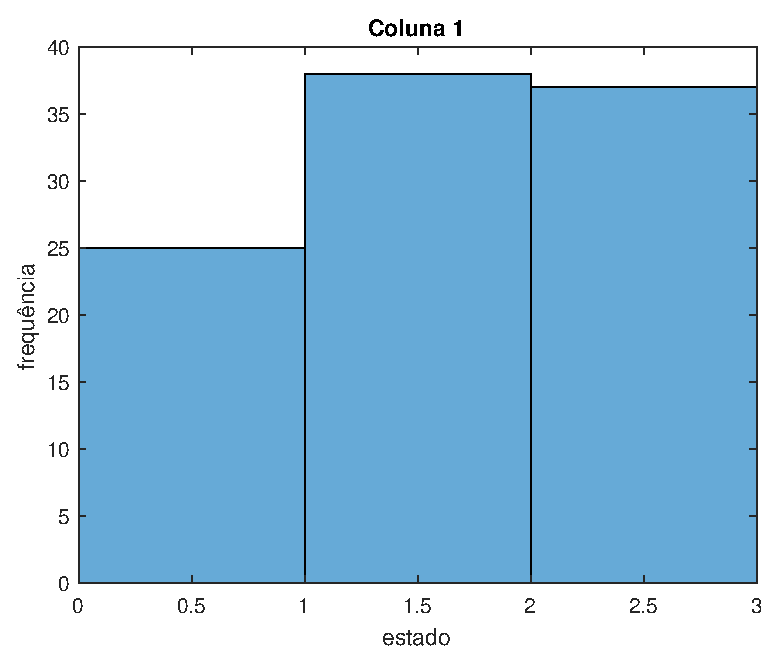
\includegraphics[width=\textwidth]{figs/ex1_1.eps}
    \end{subfigure}
    ~ 
    \begin{subfigure}[b]{0.45\textwidth}
        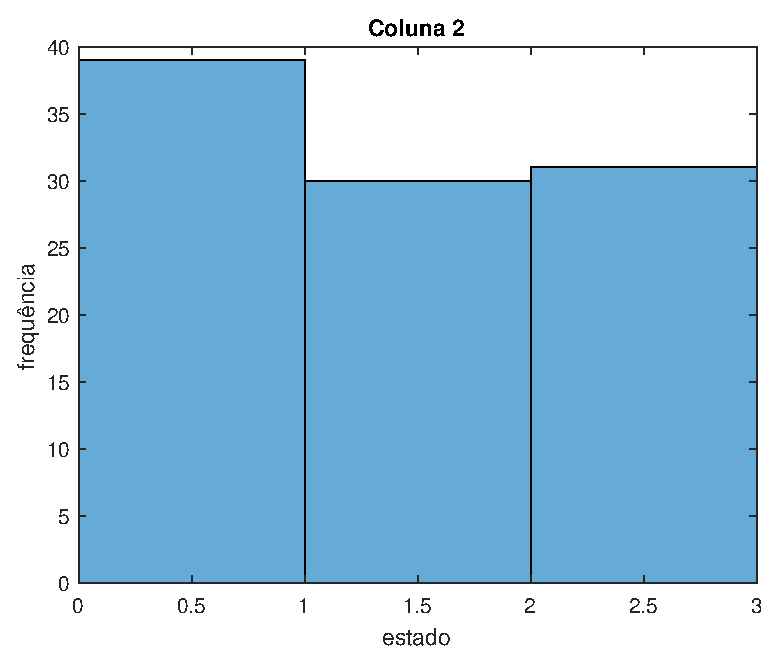
\includegraphics[width=\textwidth]{figs/ex1_2.eps}
    \end{subfigure}
\end{figure}

\begin{figure}[H]
    \centering
    \begin{subfigure}[b]{0.45\textwidth}
        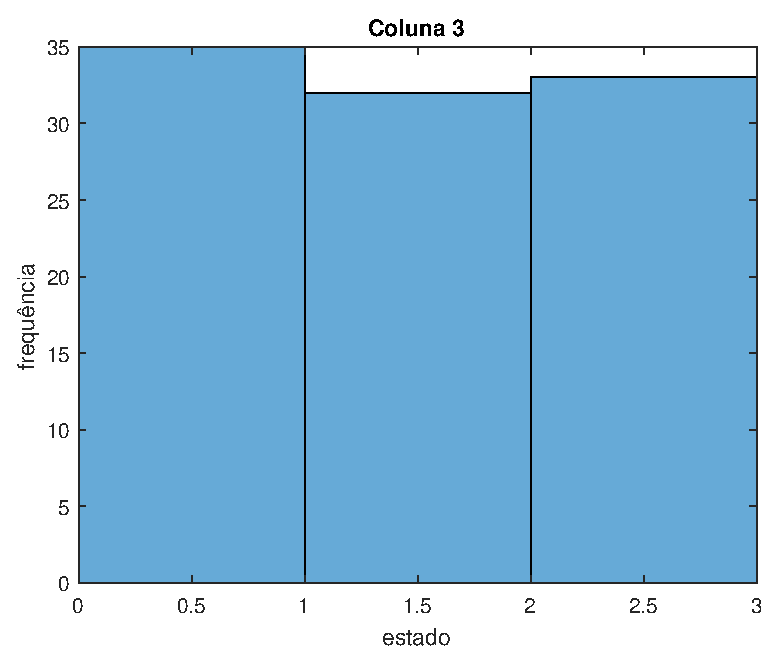
\includegraphics[width=\textwidth]{figs/ex1_3.eps}
    \end{subfigure}
    ~ 
    \begin{subfigure}[b]{0.45\textwidth}
        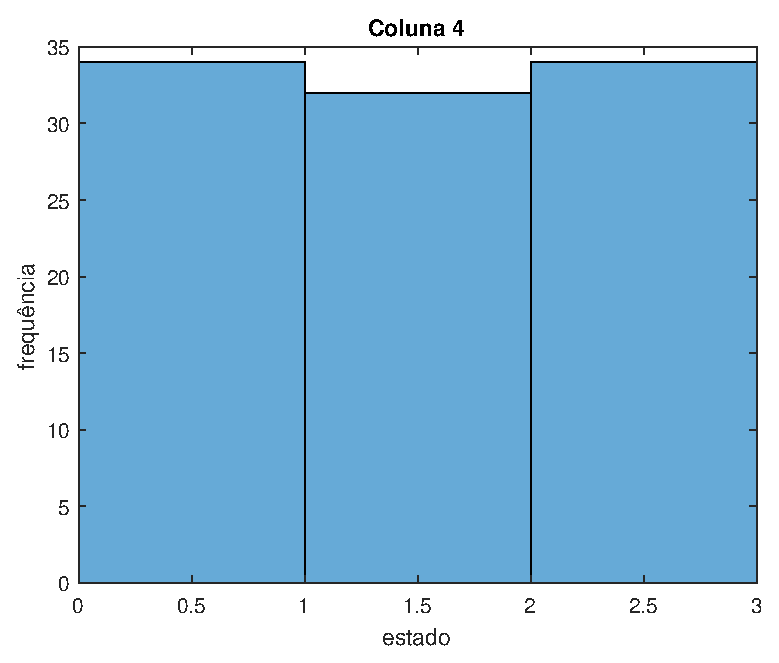
\includegraphics[width=\textwidth]{figs/ex1_4.eps}
    \end{subfigure}
\end{figure}

O código MatLab para calcular as probabilidades está abaixo:
\lstinputlisting[style=myMatlab]{matlab/ex1_d2.m}

Sabemos que o estado inicial é equiprovável para os três estados :
\begin{align*}
\textbf{p}_0 &= [0.3333 \quad 0.3333 \quad 0.3333]
\end{align*} 
E ainda:
\begin{align*}
\textbf{p}_1 &= M\textbf{p}_0 = [0.3333 \quad 0.3333 \quad
0.3333] \\
\textbf{p}_n &= M^n\textbf{p}_0 = \textbf{p}_0 = [0.3333 \quad 0.3333 \quad
0.3333]
\end{align*}

Calculamos as probabilidades pela frequência do histograma e obtemos:
\begin{align*}
\textbf{p}_0 &= [0.25 \quad 0.38 \quad 0.37] \\
\textbf{p}_1 &= [0.39 \quad 0.30 \quad 0.31] \\
\textbf{p}_2 &= [0.35 \quad 0.32 \quad 0.33] \\
\textbf{p}_3 &= [0.34 \quad 0.32 \quad 0.34]
\end{align*}

Vale observar que, conforme aumentamos o número de iterações, o estado se
aproxima para o estado estacionário $\textbf{p}_n = [0.333 \quad 0.333 \quad
0.333]$, autovetor da matriz M.
\end{exercise}

\begin{exercise}{2.a}

\begin{align*}
M = \begin{bmatrix}
0 			& \frac{1}{4} e^{-3}							& \frac{1}{4} e^{-2}										& \frac{1}{4} e^{-4}									& \frac{1}{4} e^{-1} \\
\frac{1}{4} & \frac{1}{4} (3 - e^{-1} - e^{-2} - e^{-3})	& \frac{1}{4}												& \frac{1}{4} e^{-1}									& \frac{1}{4} \\
\frac{1}{4} & \frac{1}{4} e^{-1}							& \frac{1}{4} (2 - e^{-1} - e^{-2})							& \frac{1}{4} e^{-2}									& \frac{1}{4} \\
\frac{1}{4} & \frac{1}{4}									& \frac{1}{4}												& \frac{1}{4} (4 - e^{-1} - e^{-2} - e^{-3} - e^{-4})	& \frac{1}{4} \\
\frac{1}{4} & \frac{1}{4} e^{-2}							& \frac{1}{4} e^{-1}										& \frac{1}{4} e^{-3}									& \frac{1}{4} (1 - e^{-1})
\end{bmatrix}
\end{align*}
 
O código MatLab para calcular as probabilidades está abaixo:
\lstinputlisting[style=myMatlab]{matlab/ex2_a.m}
\end{exercise}

\begin{exercise}{2.b}
Coonstruímos uma lista com os possíveis estados: $\text{list} = [1 \quad 2
\quad 3 \quad 4 \quad 5]$. Utilizamos o MatLab para fornecer um número inteiro
randômico (distribuição uniforme) entre 1 e 4:
$\text{randi}(4)$. Removemos o estadoo atual da lista: $\text{list} = [2
\quad 3 \quad 4 \quad 5]$. O número randômico será o índice do elemento que
utilizaremos como próximo candidato para estado $X(1)$: 

\begin{align}
\nonumber \text{randi}(4) &= 4 \\
\nonumber \text{list} &= [2
\quad 3 \quad 4 \quad 5] \\
\nonumber X(1) &= \text{list}(4) = 5 \\
\nonumber J(5) &< J(1) \\
\nonumber X(1) &= 5 \\
\end{align}

\begin{align}
\nonumber \text{randi}(4) &= 4 \\
\nonumber \text{list} &= [1
\quad 2 \quad 3 \quad 4] \\
\nonumber X(2) &= \text{list}(4) = 4 \\
\nonumber J(4) &< J(5) \\
\nonumber X(2) &= 4 \\
\end{align}

\begin{align}
\nonumber \text{randi}(4) &= 3 \\
\nonumber \text{list} &= [1
\quad 2 \quad 3 \quad 5] \\
\nonumber X(3) &= \text{list}(3) = 3 \\
\nonumber \text{rand} &= 0.0975 > \frac{1}{4}e^{-0.2/0.1} = 0.0338  \\
\nonumber X(3) &= 4 \\
\end{align}

\begin{align}
\nonumber \text{randi}(4) &= 2 \\
\nonumber \text{list} &= [1
\quad 2 \quad 3 \quad 5] \\
\nonumber X(4) &= \text{list}(2) = 2 \\
\nonumber \text{rand} &= 0.5469 > \frac{1}{4}e^{-0.1/0.1} = 0.092  \\
\nonumber X(4) &= 4 \\
\end{align}
\end{exercise}

\begin{exercise}{2.c}
Fazemos $[v, a] = \text{eig}(M)$. O vetor invariante é autovetor correspondente
ao autovalor 1, dividido pela soma de seus elemento:
\begin{align*}
v &= \begin{bmatrix}
0.0117 \\ 0.2341 \\ 0.0861 \\ 0.6364 \\ 0.0317 \\ 
\end{bmatrix}
\end{align*}
\end{exercise}
 
\begin{exercise}{2.d}
Calculando os fatores de Boltzmann, obtemoos:
\begin{align*}
B &= \begin{bmatrix}
e^{-5} & e^{-2} & e^{-3} & e^{-1} & e^{-4} 
\end{bmatrix} \\
B &= \begin{bmatrix}
0.0067 & 0.1353 & 0.0498 & 0.3679 & 0.0183
\end{bmatrix}
\end{align*}
Dividindo o vetor por sua soma, obtemos:
\begin{align*}
B &= \begin{bmatrix}
0.0117 & 0.2341 & 0.0861 & 0.6364 & 0.0317
\end{bmatrix}
\end{align*}
Que é o mesmo vetor invariante. 
\end{exercise}

\begin{exercise}{2.e}
O código MatLab para SA está abaixo:
\lstinputlisting[style=myMatlab]{matlab/ex2_e.m}

\begin{figure}[H]
    \centering
    \begin{subfigure}[b]{0.45\textwidth}
        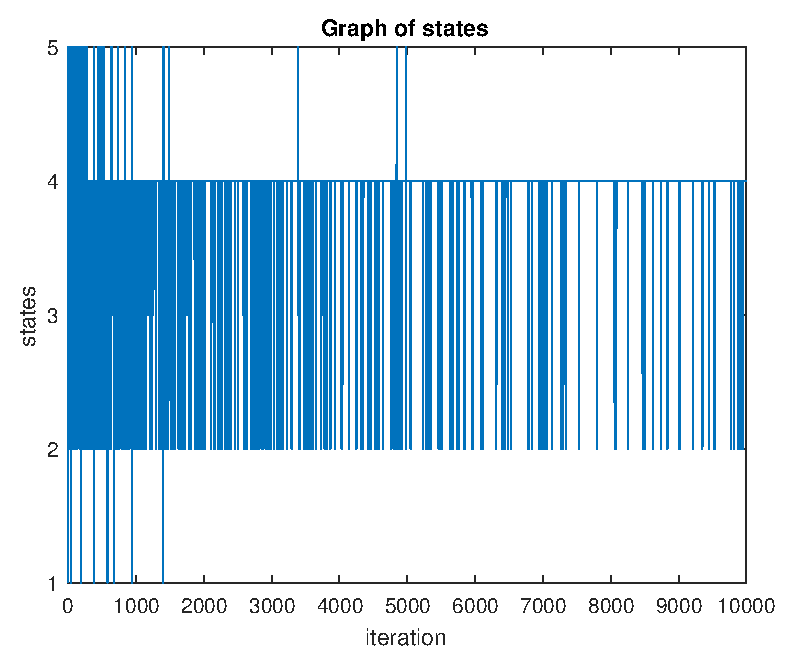
\includegraphics[width=\textwidth]{figs/ex2e_states.eps}
    \end{subfigure}
    ~ 
    \begin{subfigure}[b]{0.45\textwidth}
        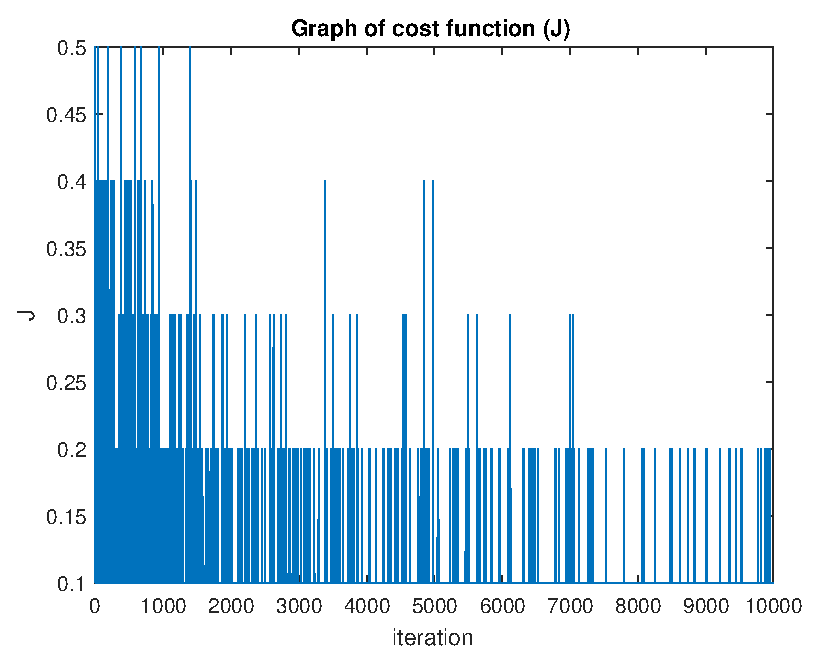
\includegraphics[width=\textwidth]{figs/ex2e_j.eps}
    \end{subfigure}
\end{figure}

\begin{figure}[H]
    \centering
    \begin{subfigure}[b]{0.3\textwidth}
        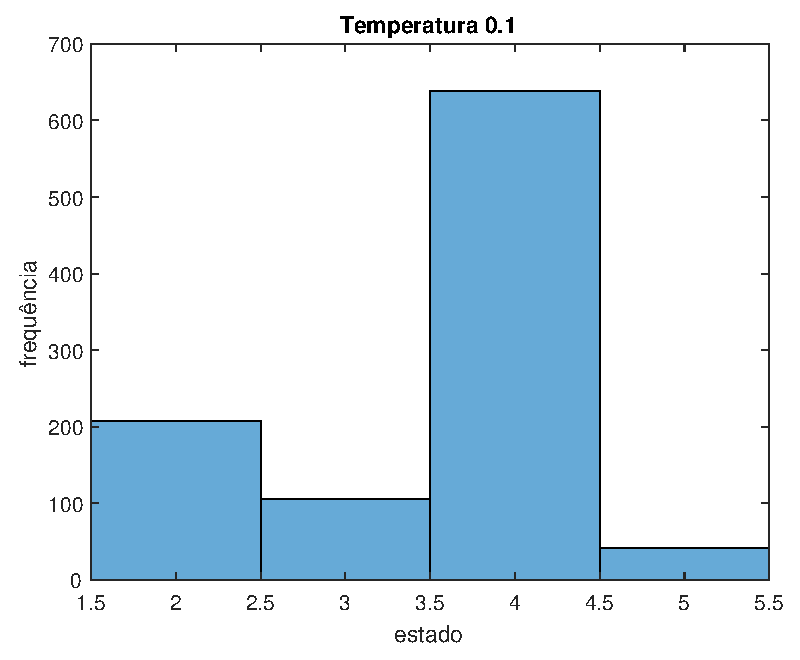
\includegraphics[width=\textwidth]{figs/ex2e_h1.eps}
    \end{subfigure}
    ~ 
    \begin{subfigure}[b]{0.3\textwidth}
        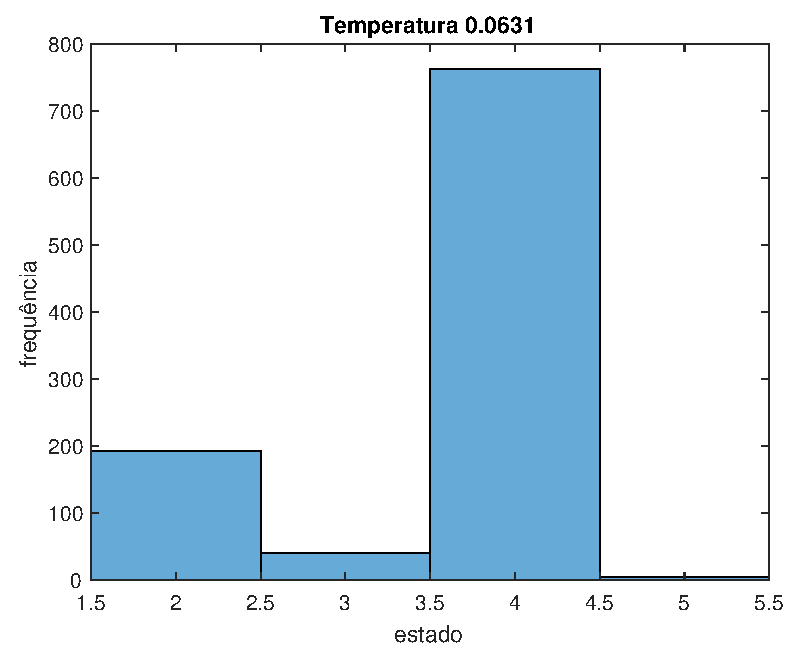
\includegraphics[width=\textwidth]{figs/ex2e_h2.eps}
    \end{subfigure}
    ~
    \begin{subfigure}[b]{0.3\textwidth}
        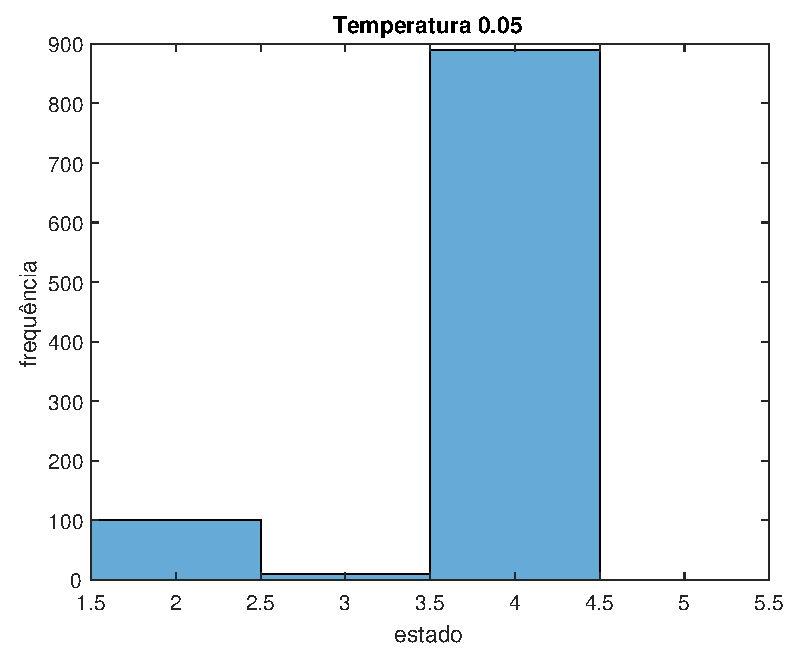
\includegraphics[width=\textwidth]{figs/ex2e_h3.eps}
    \end{subfigure}
\end{figure}

\begin{figure}[H]
    \centering
    \begin{subfigure}[b]{0.3\textwidth}
        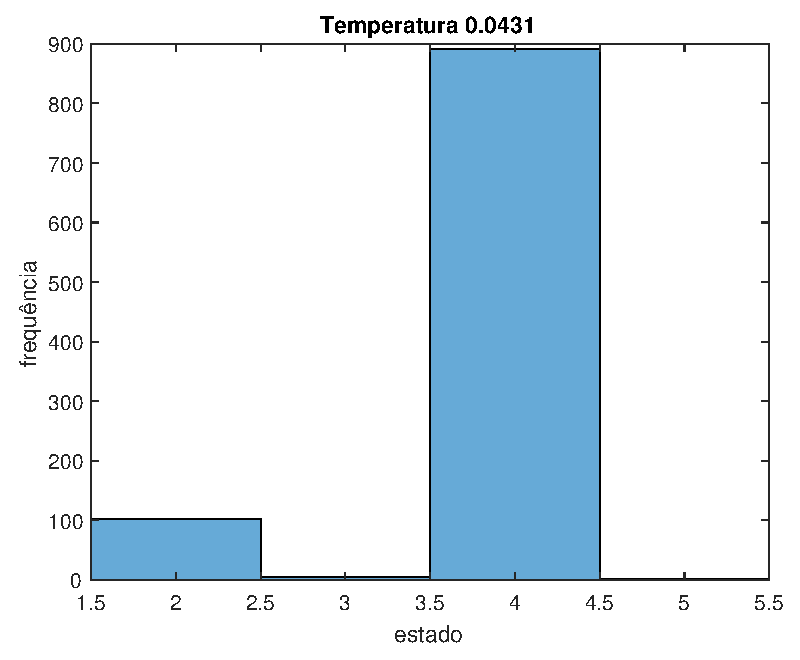
\includegraphics[width=\textwidth]{figs/ex2e_h4.eps}
    \end{subfigure}
    ~ 
    \begin{subfigure}[b]{0.3\textwidth}
        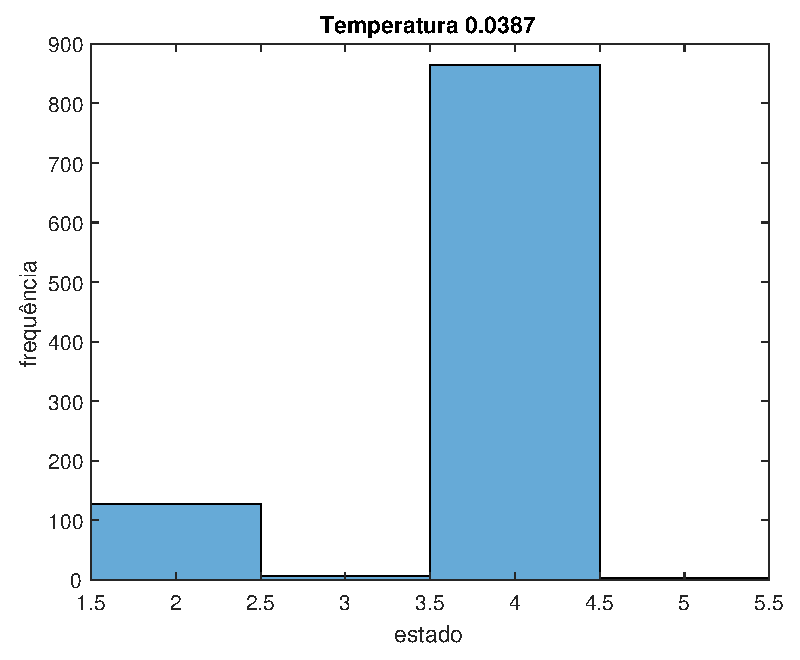
\includegraphics[width=\textwidth]{figs/ex2e_h5.eps}
    \end{subfigure}
    ~
    \begin{subfigure}[b]{0.3\textwidth}
        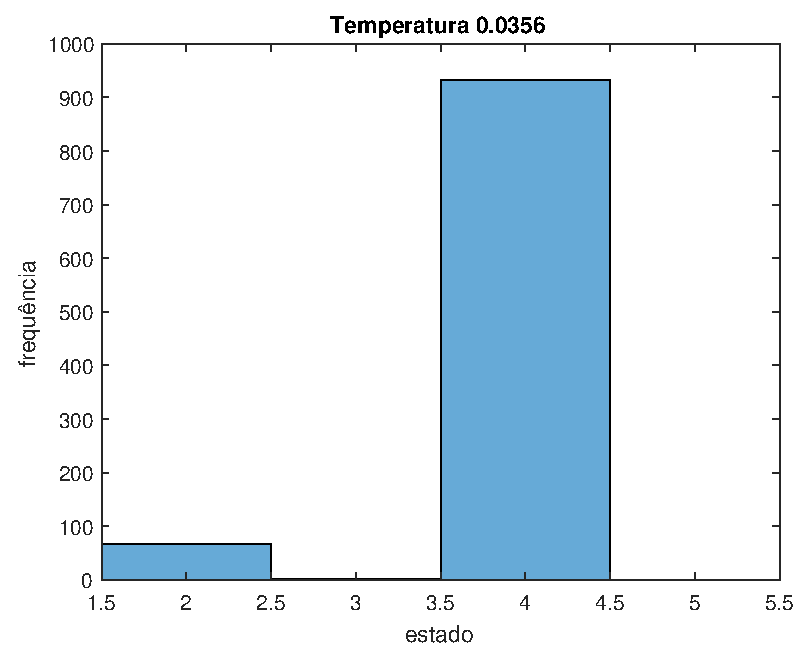
\includegraphics[width=\textwidth]{figs/ex2e_h6.eps}
    \end{subfigure}
\end{figure}

\begin{figure}[H]
    \centering
    \begin{subfigure}[b]{0.3\textwidth}
        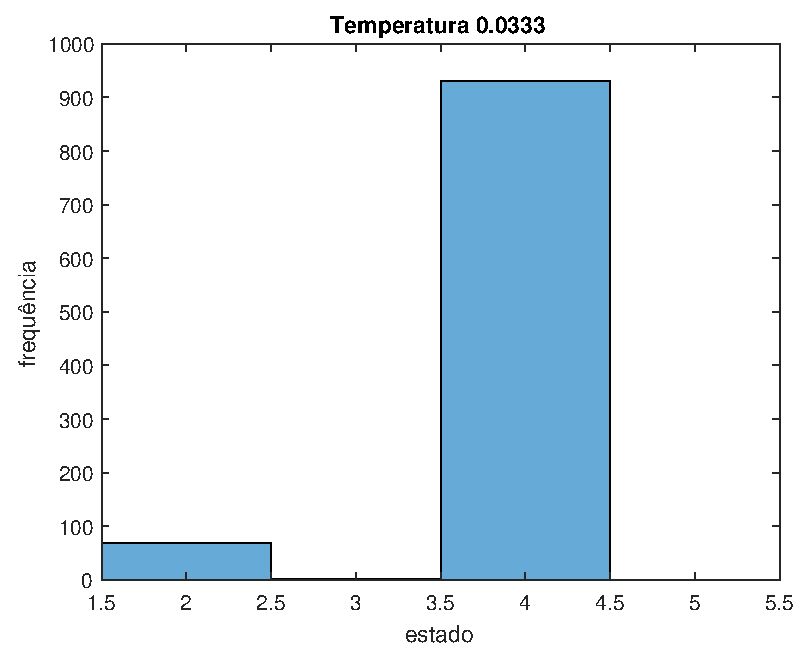
\includegraphics[width=\textwidth]{figs/ex2e_h7.eps}
    \end{subfigure}
    ~ 
    \begin{subfigure}[b]{0.3\textwidth}
        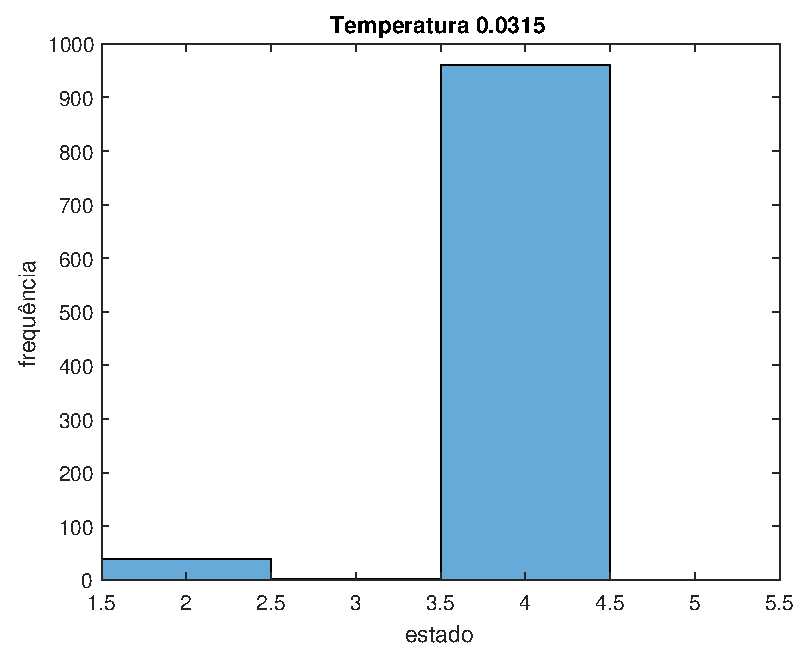
\includegraphics[width=\textwidth]{figs/ex2e_h8.eps}
    \end{subfigure}
    ~
    \begin{subfigure}[b]{0.3\textwidth}
        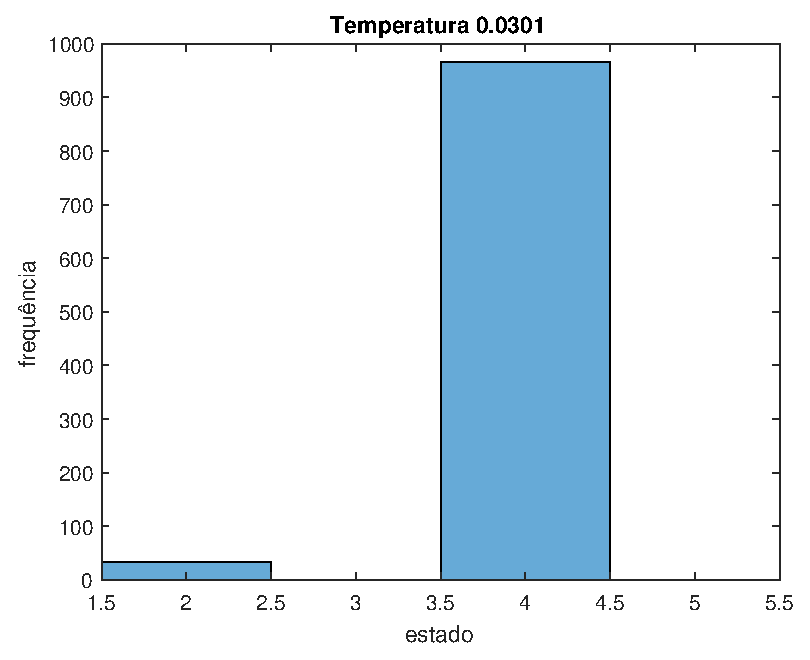
\includegraphics[width=\textwidth]{figs/ex2e_h9.eps}
    \end{subfigure}
\end{figure}

\begin{figure}[H]
    \centering
    \begin{subfigure}[b]{0.3\textwidth}
        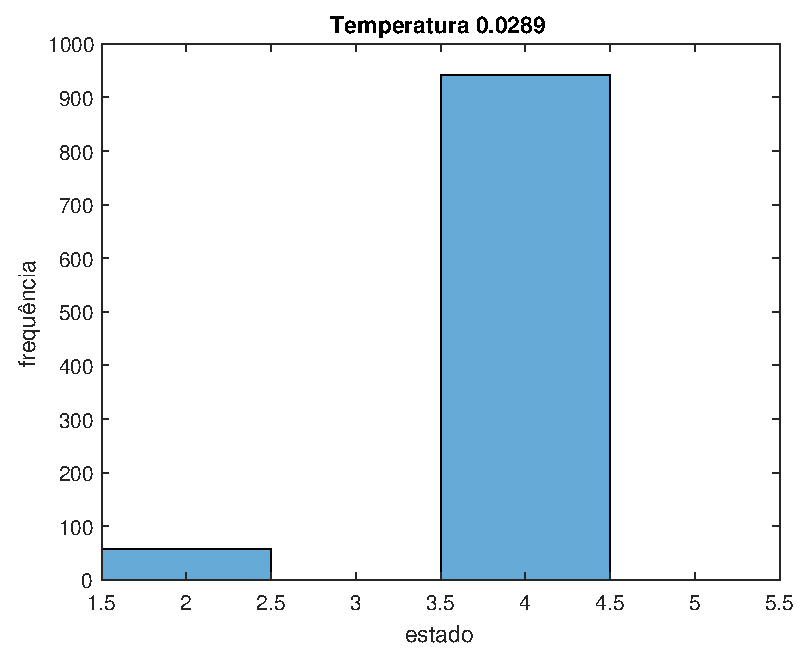
\includegraphics[width=\textwidth]{figs/ex2e_h10.eps}
    \end{subfigure}
\end{figure}
As probabilidades foram calculadas e estão abaixo:
\begin{align*}
v[1] &= \begin{bmatrix}
0.007 & 0.207 & 0.105 & 0.639 & 0.042
\end{bmatrix} \\
v[2] &= \begin{bmatrix}
0.001 & 0.192 & 0.04 & 0.763 & 0.04
\end{bmatrix} \\
v[3] &= \begin{bmatrix}
0 & 0.101 & 0.01 & 0.889 & 0
\end{bmatrix} \\
v[4] &= \begin{bmatrix}
0 & 0.102 & 0.005 & 0.892 & 0.001
\end{bmatrix} \\
v[5] &= \begin{bmatrix}
0 & 0.127 & 0.006 & 0.864 & 0.003
\end{bmatrix} \\
v[6] &= \begin{bmatrix}
0 & 0.066 & 0.002 & 0.932 & 0
\end{bmatrix} \\
v[7] &= \begin{bmatrix}
0 & 0.068 & 0.001 & 0.931 & 0
\end{bmatrix} \\
v[8] &= \begin{bmatrix}
0 & 0.038 & 0.002 & 0.96 & 0
\end{bmatrix} \\
v[9] &= \begin{bmatrix}
0 & 0.033 & 0 & 0.967 & 0
\end{bmatrix} \\
v[10] &= \begin{bmatrix}
0 & 0.058 & 0 & 0.942 & 0
\end{bmatrix} \\
\end{align*}
Inicialmente, a distribuição $v[1]$ se assemelha à probabilidade estacionária
(vetor invariante). Porém, conforme resfriamos o sistema (diminuímos a
temperatura), o estado converge para o mínimo global.
\end{exercise}

\begin{exercise}{3}
Para este exercício vamos utilizar a função Rosenbrock para N = 10:
\begin{align*}
f(\textbf{x}) = \sum_{i=1}^{N-1} 100(x_{i+1}-x_i^2)^2 + (x_i-1)^2
\end{align*}
O mínimo está em $\text{x}_\text{min}= \textbf{1}$ e $\text{J}_\text{min} =
0$. 
O código MatLab para SA está abaixo:
\lstinputlisting[style=myMatlab]{matlab/ex3.m}

A função custo:
\lstinputlisting[style=myMatlab]{matlab/J.m}

Encontramos:
\begin{align*}
\text{x}_\text{min} &= \begin{bmatrix}
0.9887 \\ 0.9877 \\ 0.9884 \\ 0.9997 \\ 1.0082 \\ 1.0121 \\ 1.0005 \\ 0.9981
\\ 1.0034 \\ 1.0511
\end{bmatrix}
\end{align*}
e $\text{J}_\text{min} = 0.3474$.

\begin{figure}[H]
    \centering
    \begin{subfigure}[b]{0.45\textwidth}
        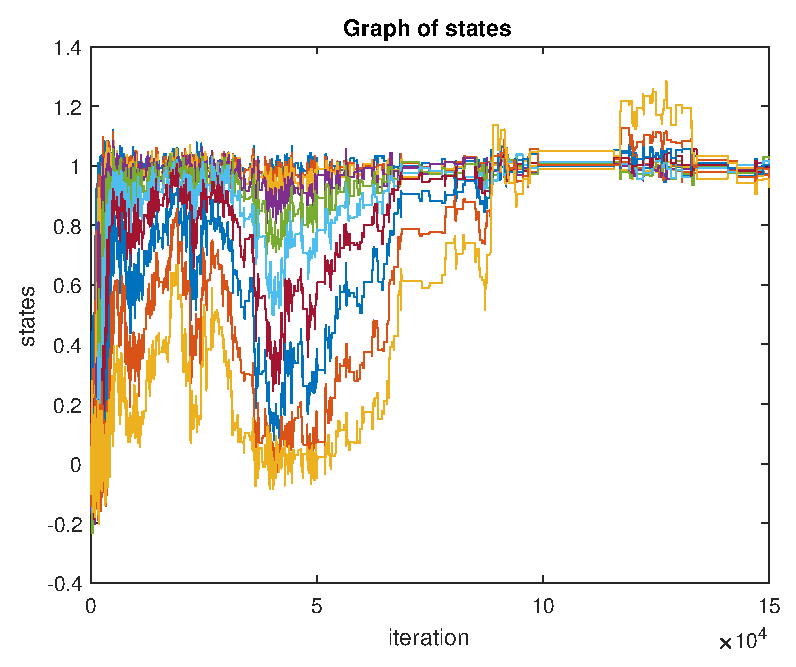
\includegraphics[width=\textwidth]{figs/ex3_states.eps}
    \end{subfigure}
    ~ 
    \begin{subfigure}[b]{0.45\textwidth}
        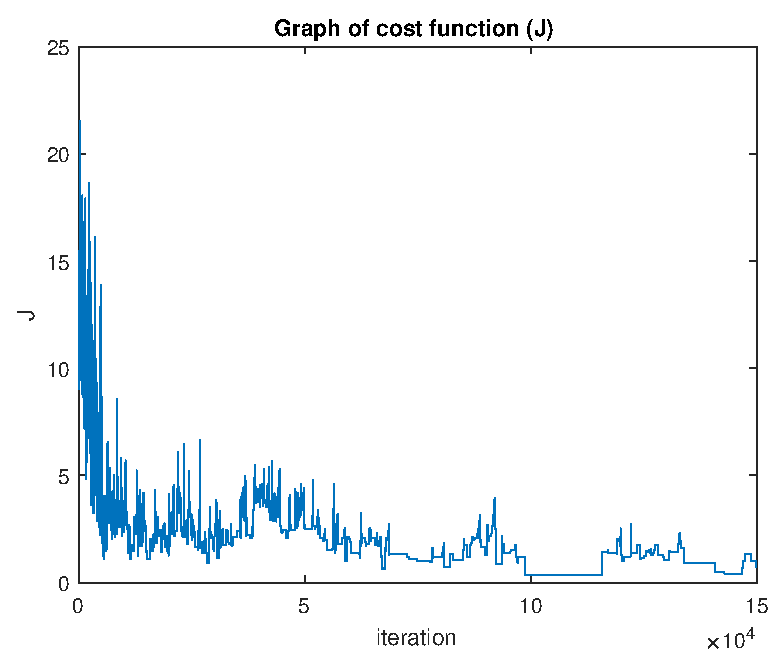
\includegraphics[width=\textwidth]{figs/ex3_j.eps}
    \end{subfigure}
\end{figure}

Verificou-se que o SA teve certa dificuldade em encontrar o mínimo global peloo
grande número de mínimos locais. O algoritmo necessitou de $5000$ iterações
para temperaturas baixas. Com um número menor de iterações (como $4000$) o
algoritmo SA não foi capaz de encontrar o mínimo. Além disso, o algoritmo é
sensível ao resfriamento (variável Temperatura), pois um resfriamento rápido ou
temperaturas iniciais baixas imopossibilitaram a convergência. 

\end{exercise}
 
\end{document}
              
